%Expositional Paper, Math 199 Fall 2022
\documentclass[12pt]{article}
\usepackage{amsmath,amssymb}
\usepackage{amsthm}
\usepackage{graphicx}
\usepackage[shortlabels]{enumitem}
\usepackage[english]{babel}
\setlength{\hoffset}{-0.33in}
\setlength{\voffset}{-1in}
\setlength{\textwidth}{6in}
\setlength{\textheight}{9in}

\renewcommand{\i}{\infty}

\newcommand{\cA}{{\mathcal A}}
\newcommand{\cB}{{\mathcal B}}
\newcommand{\cC}{{\mathcal C}}
\newcommand{\cD}{{\mathcal D}}
\newcommand{\cE}{{\mathcal E}}
\newcommand{\cF}{{\mathcal F}}
\newcommand{\cH}{{\mathcal H}}
\newcommand{\cI}{{\mathcal I}}
\newcommand{\cK}{{\mathcal K}}
\newcommand{\cL}{{\mathcal L}}
\newcommand{\cM}{{\mathcal M}}
\newcommand{\cN}{{\mathcal N}}
\newcommand{\cO}{{\mathcal O}}
\newcommand{\cP}{{\mathcal P}}
\newcommand{\cR}{{\mathcal R}}
\newcommand{\cS}{{\mathcal S}}
\newcommand{\cT}{{\mathcal T}}
\newcommand{\cU}{{\mathcal U}}
\newcommand{\cV}{{\mathcal V}}
\newcommand{\cW}{{\mathcal W}}
\newcommand{\cY}{{\mathcal Y}}

% bold letters
\newcommand{\bZ}{{\mathbb Z}}
\newcommand{\bR}{{\mathbb R}}
\newcommand{\bC}{{\mathbb C}}
\newcommand{\bT}{{\mathbb T}}
\newcommand{\bN}{{\mathbb N}}
\newcommand{\bQ}{{\mathbb Q}}

\newcommand{\bE}{{\boldsymbol E}}

\theoremstyle{definition}
\newtheorem{definition}{Definition}
\newtheorem{theorem}{Theorem}
\newtheorem{lemma}{Lemma}
\newtheorem{example}{Example}
\title{Morse Theory}
\author{Michael Huang}
\date{}

\begin{document}
\graphicspath{ {images/} }
	
\maketitle

\begin{abstract}
	Morse theory is the study of how we can extract information about the topology or geometry of a manifold from various functions (Morse functions) defined on the manifold. In this expositional paper, we will first give a quick review of important concepts from multivariable calculus then start developing the ideas of Morse theory on surfaces (2-manifolds). We will then explore an important topological invariant, the Euler Characteristic, and see how Morse theory can help us determine the Euler Characteristic of a surface without knowing what the surface looks like embedded in $\bR^3$. 
\end{abstract}

\section{Review of Multivariable Calculus}

\subsection{Critical Points and the Hessian}
We start with a general $\bR$-valued multivariable function $f(x,y)=z$. In this case, we can think of the function as taking values from the $xy$ plane and outputting a ``height'' in the $z$ direction. In full generality, we will often work with functions defined on manifolds, but in order to focus on the Morse theory part rather than the computational coordinate charts, we will often just implicitly have the coordinate charts included. 

Recall the definition of a critical point. 

\begin{definition}[Critical Point]
	Let $f:\bR^2\rightarrow \bR$ be a $\bR$-valued function in two variables. We say that a point $p_0= (a,b)\in \bR^2$ is a \textbf{critical point of $f(x,y)$} if the two following partial derivative conditions hold
	\begin{enumerate}[(a)]
		\item $\frac{\partial}{\partial x}f(x,y)|_{p_0} = 0$ (we will often shorthand $\frac{\partial}{\partial x}$ to just $\partial_x$)
		\item $\frac{\partial}{\partial y}f(x,y)|_{p_0} = 0$
	\end{enumerate}
	This definition extends in the natural way for functions of more variables, where we simply require the partial derivative in each input direction to be 0 at our critical point. 
\end{definition}

An important structure that we will need to make sure our functions are sufficiently well-behaved is the Hessian matrix. We give the definition here, and we will give some intuition as to why we need this when we go on to define Morse functions. 
\begin{definition}[Hessian Matrix]
	Let $f:\bR^2\rightarrow \bR$ be as above and $p_0$ a critical point of $f$. We define the \textbf{Hessian} $\cH_f(p_0)$ of $f$ at $p_0$ to be the matrix of mixed partial derivatives evaluated at $p_0$, i.e.
	\begin{center}
		$\cH_f(p_0) = \begin{pmatrix}
			&\frac{\partial^2}{\partial x^2}f(x,y)|_{p_0} & \frac{\partial^2}{\partial x \partial y}f(x,y)|_{p_0}&  \\
			\\
			&\frac{\partial^2}{\partial y \partial x}f(x,y)|_{p_0} & \frac{\partial^2}{\partial y^2}f(x,y)|_{p_0} &
			\end{pmatrix}$
	\end{center}
	% \begin{center}
	% 	$\cH_f(p_0) = \begin{pmatrix}
	% 		&(\partial_x)^2 f(x,y)|_{p_0} &  \partial_x \partial_y f(x,y)|_{p_0}&  \\
	% 		\\
	% 		&\partial_y \partial_x f(x,y)|_{p_0} & (\partial_y)^2f(x,y)|_{p_0} &
	% 		\end{pmatrix}$
	% \end{center}
\end{definition}

\noindent
The Hessian itself is actually not as important as the determinant of the Hessian matrix, which in the $2\times 2$ case is simply given by 
\begin{center}
	$|\cH_f(p_0)| = [\frac{\partial^2}{\partial x^2}f \frac{\partial^2}{\partial y^2}f - (\frac{\partial^2}{\partial x \partial y}f)^2]_{p_0}$
\end{center}
Notice that since partial derivatives commute, the Hessian is actually a symmetric matrix, as $\frac{\partial^2}{\partial x \partial y}f = \frac{\partial^2}{\partial y \partial x}f$. 

We can now give another important definition which characterizes the critical points of a function. 
\begin{definition}[(Non-)Degenerate Critical Point]
	Let $p_0$ be a critical point of $f$. We say that $p_0$ is a \textbf{degenerate critical point} of $f$ if $|\cH_f(p_0) = 0|$, that is, if the determinant of the Hessian of $f$ at $p_0$ is 0. We say that $p_0$ is non-degenerate if the determinant is non-zero. 
\end{definition}

\noindent
Roughly speaking, the idea here is that if the determinant of the Hessian is 0 at $p_0$, there exists some direction in our input space for which moving along that direction at $p_0$ we don't change our $z$ value. This leads to us having ``non-isolated'' critical points, where instead we might have a line of critical points. This type of behavior is what we want to avoid when we define Morse functions. 

\noindent
We should hope that this degeneracy characterization is basis independent, otherwise we would have to explicitly find a coodinate system that satisfies this condition, defeating the purpose of Morse theory all together. Indeed, we have the following theorem.

\begin{theorem}
	Let $(x,y)$ and $(u,v)$ be two different coordinate systems for our input space of $f$. If $q_0$ is a critical point of $f$ in the $(x,y)$ basis and $p_0$ is the corresponding point in the $(u,v)$ basis, then we have that 
	\begin{center}
		$|\cH_f(q_0)| \neq 0$ if and only if $|\tilde{\cH_f}(p_0)| \neq 0$. 
	\end{center}
\end{theorem}
\begin{proof}
	Let $J$ denote the Jacobian of the coordinate transformation $(x,y)\mapsto (u,v)$. Then, we have that $\tilde{\cH_f}(q_0) = J^{-1} \cH_f(p_0) J$. Since $J$ is the Jacobian of a coordinate transformation, we know that $|J|\neq 0$, and similarly, $|J^{-1}|\neq 0$. Now, from linear algebra, we get that $|\tilde{\cH_f}(p_0)| = |J^{-1}\cH_f(q_0)J|= |J^{-1}||\cH_f(q_0)||J|$ where our result clearly follows. 
\end{proof}
\pagebreak
\section{Morse Theory on Surfaces}
The first main result of Morse theory characterizes the local geometry of our surface just by looking at the critical points of a (Morse) function defined on the surface. 

\begin{theorem}
	Let $f:\bR^2 \rightarrow \bR$ be a function of two variables with a non-degenerate critical point $p_0$. Then, we can choose appropriate local coordinates $(u,v)$ such that the function $f$ expressed in the $(u,v)$ basis takes one of the following standard forms:
	\begin{enumerate}[(i)]
		\item $f = u^2+v^2+f(p_0)$
		\item $f = u^2 - v^2 + f(p_0)$
		\item $f = -u^2 -v^2 + f(p_0)$
	\end{enumerate}
\end{theorem}
\noindent
As a quick remark, all the surfaces we will be doing Morse theory on will have some regularity condition, say, locally diffeomorphic to $\bR^2$, so it makes sense to even talk about the Morse lemma on surfaces. In other words, for some 2-manifold $M\subset \bR^3$ we can just compose our ``Morse function'' $h:M\rightarrow \bR$ and a local coordinate chart $X:\bR^2 \rightarrow M$ to get the function $f:= h\circ X: \bR^2 \rightarrow \bR$. 

Before we can give the proof of the Morse Lemma, we give a few useful results. 
\subsection{Preliminaries to the Morse Lemma}

We start with a simple lemma 
\begin{lemma}\label{lemma:1} 
	If $f(x,y)$ is a $\bR-$valued function such that $f(0,0)= 0$, then there exist functions $h(x,y)$ and $g(x,y)$ such that $f(x,y) = xg(x,y) + yh(x,y)$ in some neighborhood of $(0,0)$ and such that $\partial_xf(0,0) = g(0,0)$ and $\partial_y f(0,0)=h(0,0)$.
\end{lemma}

\begin{proof}
	Let $f(x,y)$ be given as above. Notice, $f(x,y) = \int_0^1 \frac{df(xt,ty)}{dt}dt$ for a fixed parameter $t$. This equality follows from a simple application of the fundamental theorem of calculus. Now, expanding our integrand by using chain rule, we get 
	\begin{center}
		$f(x,y) = \int_0^1 x \partial_x f(xt,yt) + y\partial_y f(xt,yt) dt$
	\end{center}
	Since our integration variable is $t$, we can pull out the $x$ and $y$ to get
	\begin{center}
		$f(x,y) = x\int_0^1 \partial_xf(xt,yt)dt + y \int_0^1 \partial_y f(xt,yt)dt$
	\end{center}
	so we can take $g(x,y):= \int_0^1 \partial_xf(xt,yt)dt$ and $h(x,y):= \int_0^1 \partial_yf(xt,yt)dt$ and we get that $g(0,0) = \partial_xf(0,0)$ (and similarly for $h(0,0)$). 
\end{proof}
We pick up this result in order to have a better local description of our function and its derivatives, something that we will apply multiple times in our proof of the Morse lemma. 

Here is another useful lemma. 

\begin{lemma}
	Let $f:\bR^2 \rightarrow \bR$ be a function of two variables with a non-degenerate critical point $p_0$. Then, there exists a local coordinate system $(x,y)$ such that $\frac{\partial^2 f}{\partial x^2}|_{p_0} \neq 0$. 
\end{lemma}

\begin{proof}
	Let $(u,v)$ be any local coordinate system around $p_0$. We can do casework. If $\frac{\partial^2 f}{\partial u^2}|_{p_0} \neq 0$, we are done, so we only need to consider two cases, namely $\partial_u^2f(p_0) = 0$ and $\partial_v^2 f(p_0)\neq 0$, or $\partial_u^2f(p_0) = 0$ and $\partial_v^2 f(p_0) = 0$. 

	Case 1: $\partial_v^2 f(p_0)\neq 0$

	In this case, we can simply use the coordinate system $(x,y) = (v,u)$ and we have $\partial_x^2f(p_0) = \partial_v^2f(p_0)$. 

	Case 2: $\partial_v^2f(p_0) =0$

	For this case, we will use the non-degeneracy condition. Namely, we have that 
	\begin{center}
		$\cH_f(p_0) = \begin{pmatrix}
			0 & a  \\
			a & 0 
			\end{pmatrix}$
	\end{center}
	and $|\cH_f(p_0)| = 0\cdot 0 - a^2$, where $a = \partial_{uv}^2f(p_0)$. Non-degeneracy tells us that $a \neq 0$, so consider the coordinate system $(x,y) = (u-v,u+v)$. The Jacobian for this transformation from $(u,v) \rightarrow (x,y)$ is given by 
	\begin{center}
		$J = \begin{pmatrix}
			1 & -1  \\
			1 & 1 
			\end{pmatrix}$
	\end{center}
	The Hessian $\bar{\cH}$ in the $(x,y)$ coordinate system is then given by 
	\begin{center}
		$\bar{\cH} = J^T \cH J = \begin{pmatrix}
			2a & 0  \\
			0 & -2a 
			\end{pmatrix}$
	\end{center}
	which tells us that $\partial_x^2f(p_0) = 2a \neq 0$. 
\end{proof}
This lemma will essentially be used to make sure we are not dividing by 0 at any point in our construction. 

\subsection{The Morse Lemma}

This section will be dedicated to giving the proof of the Morse Lemma. Recall the statement

\noindent
\textbf{Theorem 2} (Morse Lemma)\textbf{.}
	Let $f:\bR^2 \rightarrow \bR$ be a function of two variables with a non-degenerate critical point $p_0$. Then, we can choose appropriate local coordinates $(u,v)$ such that the function $f$ expressed in the $(u,v)$ basis takes one of the following standard forms:
	\begin{enumerate}[(i)]
		\item $f = u^2+v^2+f(p_0)$
		\item $f = u^2 - v^2 + f(p_0)$
		\item $f = -u^2 -v^2 + f(p_0)$
	\end{enumerate}
\begin{proof}
	We start by choosing a local coordinate system around $p_0$ such that $\partial_x^2f(p_0) \neq 0$, given to us by Lemma 2. Without loss of generality, we can assume $p_0 = (0,0)$ and $f(p_0)=0$, otherwise, just shift everything by a constant. Now, applying Lemma 1, we write $f(x,y) = xg(x,y) + yh(x,y)$ for some neighborhood around $p_0$, where $\partial_xf(0,0) = g(0,0)$ and $\partial_y f(0,0) = h(0,0)$. Since $p_0 = (0,0)$ is a critical point of $f$, we get that $g(0,0) = h(0,0) = 0$, so we can apply Lemma 1 once again to $g$ and $h$ separately, giving us $g(x,y) =x h_{11}(x,y) + yh_{12}(x,y)$ and $h(x,y) = xh_{21}(x,y)+yh_{22}(x,y)$ for some functions $h_{ij}$. All of this is happening in (smaller and smaller) neighborhoods around $(0,0)$, so we can always just take the largest neighborhood such that these forms still hold.
	
	Now, plugging everything back in, we get $f(x,y) = x^2h_{11} + xy(h_{12}+h_{21})+ y^2h_{22}$. Defining $H_{11}:= h_{11}, H_{12} := \frac{1}{2}(h_{12}+h_{21}),$ and $H_{22}:= h_22$, we get a slightly more suggestive form $f(x,y) = x^2 H_{11}+ 2xyH_{12}+ y^2H_{22}$. Taking two $\partial_x$ derivatives, we get that $\partial_x^2 f(0,0)= 2H_{11} \neq^! 0$, so we are free to divide by $H_{11}$, where we used lemma 2 at $\neq^!$. This allows us to define a new coordinate system given by $u = \sqrt{|H_{11}|}\left(x + \frac{H_{12}}{H_{11}}y\right)$. For now, we do not change $y$. Note that since $H_{11} \neq 0$ in our neighborhood, $u$ and $y$ are never linearly dependent, meaning we actually have a complete coordinate system. 

	We want to rewrite $f$ in this new coordinate, so we can square $u$ to get 
	\begin{center}
		$u^2= 
		\left\{
			\begin{array}{lr}
				H_{11}x^2+2H_{12}xy+\frac{H_{12}^2}{H_{11}}y^2, & \text{if } H_{11}>0\\
				-H_{11}x^2-2H_{12}xy-\frac{H_{12}^2}{H_{11}}y^2, & \text{if } H_{11}<0\\
			\end{array}
		\right\}$
\end{center}
	After some simple algebraic manipulation, this lets us write 
	\begin{center}
		$f= 
		\left\{
			\begin{array}{lr}
				u^2+\left(H_{22}-\frac{H_{12}^2}{H_{11}}\right)y^2, & \text{if } H_{11}>0\\
				-u^2+\left(H_{22}-\frac{H_{12}^2}{H_{11}}\right)y^2, & \text{if } H_{11}<0\\
			\end{array}
		\right\}$
\end{center}
	Essentially what we have done here is ``throw away'' a lot of unimportant (geometric) data and focus more on the sign of the top right entry of the Hessian, $H_{11}$.
	Notice, the coefficient of $y^2$ can actually be written as 
	$H_{22}-\frac{H_{12}^2}{H_{11}}=\frac{1}{H_{11}}\left(H_{11}H_{22}-H_{12}H_{21}\right)$. By our definition of $H_{ij}$, we see that $H_{11} = 2\partial_x^2f,H_{12} = 2\partial_x\partial_yf,$ and $H_{22} = 2\partial_y^2f$. Thus 
	\begin{center}
		$\frac{1}{H_{11}}\left(H_{11}H_{22}-H_{12}H_{21}\right) = \frac{|\cH_f|}{4H_{11}}$ 
	\end{center}
	By our non-degeneracy assumption, the numerator is non-zero and our choice of coordinates tells us that $H_{11}\neq0$, so we can finally define $v = \sqrt{|\frac{|\cH_f|}{4H_{11}}|}y$. Rewriting $f$, we get the final Morse form we were promised.
	\begin{center}
		$f= 
		\left\{
			\begin{array}{lr}
				u^2+v^2, & \text{if } H_{11}>0, |\cH_f|>0\\
				u^2-v^2, & \text{if } H_{11}>0, |\cH_f|<0\\
				-u^2+v^2, & \text{if } H_{11}<0, |\cH_f|<0\\
				-u^2-v^2, & \text{if } H_{11}<0, |\cH_f|>0\\
			\end{array}
		\right\}$
	\end{center}
	Again, we have essentially thrown away all the data about the local geometry of our surface and just honed in on the signs of the entries of our (diagonalized) Hessian of our function. In other words, since the Hessian has non-zero determinant, it can be diagonalized by applying a unitary transformation, but if we allow non-linear invertible transformations as well, we can get our Hessian to be of the form 
	\begin{center}
		$\tilde{\cH_f} = \begin{pmatrix}
			\pm 1 & 0  \\
			0 & \pm 1 
			\end{pmatrix}$
	\end{center}
	and our Morse form exactly encapsulates the signs of the entries. As such, we can also define the \textbf{Morse index} of each critical point $p_0$ to be the number of negative signs in the diagonalized Hessian at $p_0$. For a surface, the Morse index takes values in $\{0,1,2\}$ and will be very important in our discussion of handle decomposition in the future. 
	
	As a final remark, notice that the second and third standard form are equivalent up to swapping coordinates $(u,v)\mapsto (v,u)$, so we really only have three distict Morse forms. 
\end{proof}


\subsection{Basic Results}

One immediate but important consequence of the Morse Lemma is given as follows. 

\begin{theorem}
	A Morse function $f:M\rightarrow \bR$ defined on a closed surface $M$ can only have a finite number of critical points.
\end{theorem}

\begin{proof}
	We split this proof into two main steps: 

	Step 1:
    The first part of this proof will be to show that the set of critical points of $f$ is compact. Consider the set $S = \bigcup p_i$, of all critical points on $M$. We claim that $\bar{S} = S$, that is, $S$ is closed. We get that $S\subseteq \bar{S}$ for free, so we we just need to show inclusion in the other direction. Let $x \in \bar{S}$. Since $S$ is dense in $\bar{S}$, for any $\varepsilon > 0$, we can find some $p_i$ such that $d(p_i,x)<\varepsilon$. By looking at the sequence of $p_{i_n}$ such that $d(p_{i_n},x)\leq \frac{1}{2^n}$, we can find a sequence of critical points converging to $x$. We claim this means $x$ must be a critical point and thus in $S$. Indeed, since $f$ is differentiable with continuous derivative, $\frac{\partial f}{\partial x^i}(p_{i_n}) = 0$ for all $p_{i_n}$ implies that $\frac{\partial f}{\partial x^i}(x) = 0$, so $x \in S$. Now, we know $S$ is a closed subset of a compact space ($M$), so $S$ itself must be compact. 
	
	Step 2:
	Now we can prove our desired result. For each $p_i \in S$, we define $U_i$ to be the (open) neighborhood around $p_i$ such that $f$ takes one of the three standard ``Morse'' forms, promised by the Morse Lemma. Clearly the $U_i$ form an open cover of $S$, so since $S$ is compact, there is some finite subset $\{p_{\alpha_1}, ... ,p_{\alpha_n}\}$ of critical points such that the $U_{\alpha_i}$ cover S. However, we claim now that $f$ can only have $n$ critical points in $S$. Indeed, by the Morse lemma, each $U_{\alpha_i}$ has a local coordinate system $(x,y)$ on which $M = \pm x^2 \pm y^2 +c$, so there is exactly one critical point in each $U_{\alpha_i}$, meaning the total number of critical points is equal to the total number in the finite subcover, $n$.
\end{proof}
\noindent
There are countlessly many more results we can prove just by knowing the Morse lemma, but in order to keep this section relatively brief, we will just list a few interesting ones without giving a proof. 

\begin{theorem}
	Let $M\subset \bR^3$ be a compact surface. If there exists a morse function $f:M\rightarrow \bR$ with exactly two non-degenerate critical points, then $M$ is diffeomorphic to the 2-sphere, $S^2$. 
\end{theorem}

\begin{theorem}
	A non-degererate critical point must be isolated, that is, there exists some open neighborhood around the critical point for which there exists no other critical points. 	
\end{theorem}

\subsection{Handle Decomposition}

One natural question that comes up at this point is if we can do everything up to this point backwards, that is, if we are given a Morse function and the Morse index of each critical point, can we somehow use the data to reconstruct what our original surface looked like?

To answer this, we need to develop the thoery of handle decomposition. We start by giving some definitions and a useful lemma. 

\begin{definition}[Sublevel Set]
	Let $f:M\rightarrow \bR$ be a morse function defined on a connected surface $M$. We define the \textbf{sublevel set} $M_t$ of $M$ at $t$ as the set of all points in $M$ for which $f$ takes a value of less than or equal to t. Explicitly, 
	\begin{center}
		$M_t = \{p\in M: f(p)\leq t\}$
	\end{center}
	We define the \textbf{level set} as the obvious extension
	\begin{center}
		$L_t = \{p\in M: f(p)= t\}$
	\end{center}
\end{definition}

\noindent
This next definition is completely independent of Morse theory, but can be helpful for notational clarity. 

\begin{definition}[Critical Value]
	Let $f$ be any $\bR-$valued function which admits critical point(s). We say that $c_0 \in \bR$ is a \textbf{critical value} if $f(p_0) = c_0$ for some critical point $p_0$. 
\end{definition}
\noindent 
Now we give an important lemma that will describe our surface behaves between critical values of a morse function. 
\begin{lemma} Let $f:M\rightarrow \bR$ be a Morse function and let $[a,b]\subset \bR$ be an interval. If $f$ has no critical values in $[a,b]$, then $M_{[a,b]}\cong f^{-1}(a) \times [0,1]$. 
\end{lemma}

\begin{proof}
      Let $X$ be a gradient-like vector field for $f$. Since $f$ has no critical values in $[a,b]$, we can consider a new vector field $Y$ on $M_{[a,b]}$ defined by $Y = \frac{X}{X\cdot f}$. Intuitively, we are normalizing $X$ such that the integral curves of $Y$ are unit speed under the ``metric'' defined by $f$. We can verify this. Let $p \in f^{-1}(a)$ (in fact, this $p$ can be chosen to be anywhere on $M_{[a,b]}$) and let $c_p(t)$ denote the integral curve of $Y$ through $p$. Notice, $\frac{d}{dt}f(c_p(t)) = \frac{d}{dt}c_p(t)\cdot f = Y|_{c(t)}\cdot f = \frac{X\cdot f}{X \cdot f} = 1$, so we can write $f(c_p(t)) = t + C$ for some constant $C$. Since we defined $c_p(0) = p$ and $f(p)=a$, we have that $f(c_p(0)) =a $ and we get that $f(c_p(t))=t+a$, so $f(c_p(b-a)) = b-a+a = b$. What we have just shown is that each integral curve of $Y$ starting at a point on $f^{-1}(a)$ reaches some point in $f^{-1}(b)$. By the uniqueness of integral curves, each point on $f^{-1}(a)$ reaches exactly one point on $f^{-1}(b)$. In fact, we claim that this construction provides a bijection between the points in $f^{-1}(a)$ and $f^{-1}(b)$. Injectivity has already been shown, and to see surjectivity, we can repeat the steps above except with points starting at $f^{-1}(b)$ with integral curves of $Y = -\frac{X}{X\cdot f}$. What we get in this case is that each integral curve starting at a point on $f^{-1}(b)$ reaches a point on $f^{-1}(a)$, so the points on $f^{-1}(a)$ are in bijection with the points on $f^{-1}(b)$ by considering the family of integral curves defined by $Y = \pm\frac{X}{X\cdot f}$.

      Now consider the map $h:f^{-1}(a)\times [0,b-a] \rightarrow M_{[a,b]}$ defined by $h(p,t) = c_p(t)$. We claim this is a diffeomorphism. By the theory of differential equations, this map is smooth and if an inverse exists, is smooth as well, so we just have to show this map is bijective. First, we will show $h$ is surjective. Indeed, for any point $p \in M_{[a,b]}$, we can consider the integral curve $c_p(t)$ of $Y = -\frac{X}{X\cdot f}$. By the analysis above, there is some $q \in f^{-1}(a)$ such that $c_q(t_0)=p$ for some $t_0$. We almost get injectivity for free from the uniqueness of integral curves, but we have to make sure the curve cannot have periodic behavior. However, this follows from the fact that since $f$ has no critical values in $[a,b]$, $f$ composed with each integral curve must be monotonic, so cannot exhibit periodic behavior. Thus $h$ is in fact bijective, so is a diffeomorphism. 
\end{proof}
	Essentially, this lemma tells us that in any interval not containing critical values, our surface is differomorphic to just taking the level set at one endpoint of our interval and ``raising it up" with respect to our morse function. 

	Now, we return to the question we started this section with by developing the theory of Handle decompostion. As we know from our discusstion above, each critical point of a Morse function can be characterized into one of three categories, depending on its Morse index. We can consider how our surface behaves before and after this critical point. To make this discussion easier, we can introduce the ``shapes'' we will attach along their \textbf{attachment boundaries} to our sublevel sets in order to create our manifold. These 2-manifolds are often called \textbf{$n-$handles} and are described as follows. 
	
	\begin{definition}[$n-$handle] 
	\end{definition}
		
	\begin{enumerate}

	\item \textbf{0-Handle}\\
		  A 0-handle $H_0$ is given by $H_0 \cong D^0 \times D^2$, with attachment boundary $\partial_\cA H_0 \cong \partial D^0 \times D^2 \cong \emptyset$. 
		  \begin{center}
				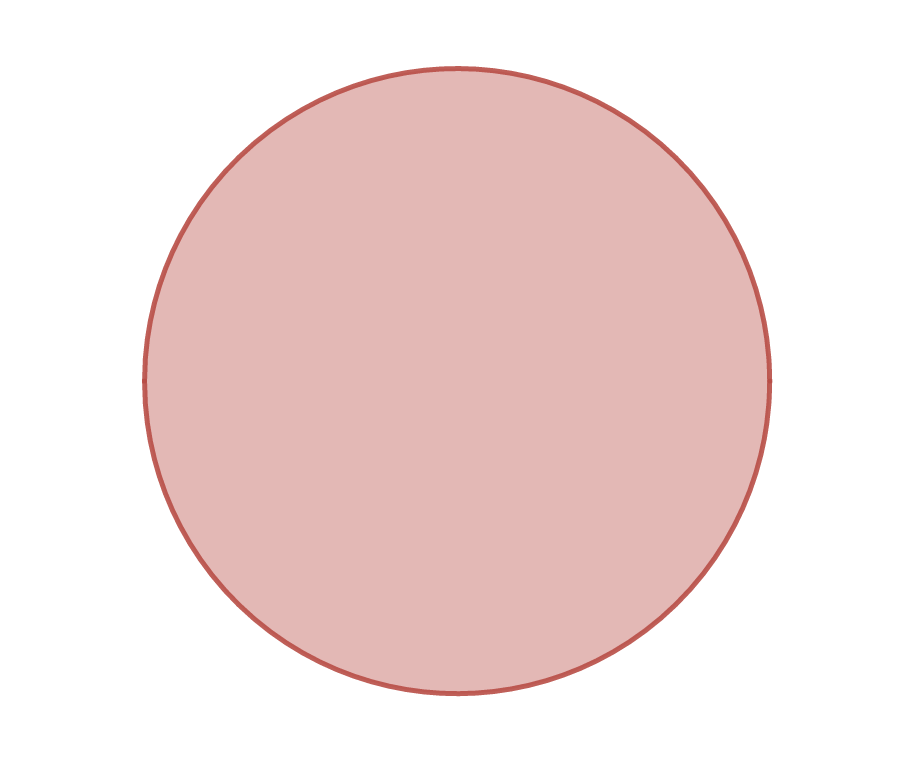
\includegraphics[scale=0.4]{H_0.png}\\
				$H_0$
				
		  \end{center}
	\item \textbf{1-Handle}\\
		  A 1-handle $H_1$ is homeomorphic to the cartesian product of two intervals, $H_1 \cong D^1\times D^1$ with attachment boundary $\partial_\cA H_1 \cong \partial D^1 \times D^1 \cong D^1 \sqcup D^1$. 
		  \begin{center}
				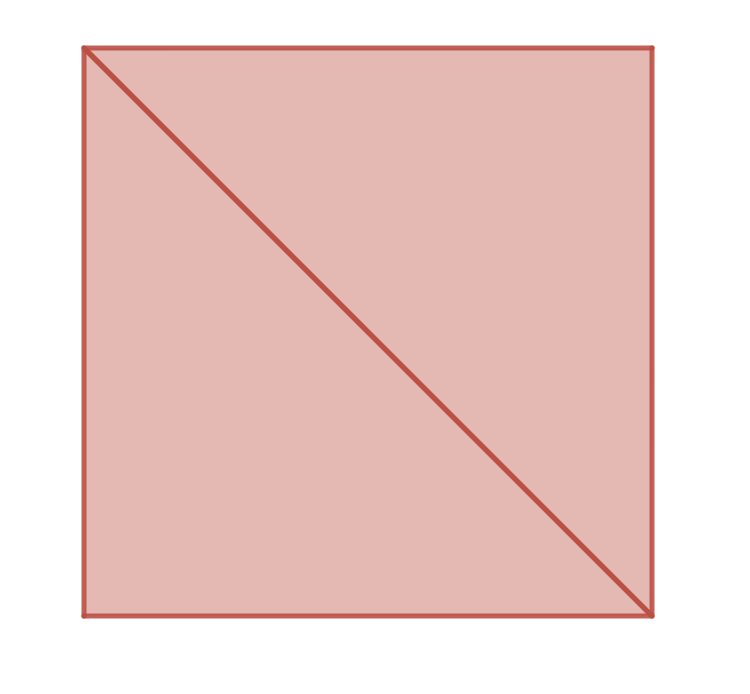
\includegraphics[scale=0.5]{square.png} \\
				$H_1 \cong D^1\times D^1$

				
\includegraphics[scale = 0.5]{D_H_1.png}\\
				$\partial_\cA H_1 \cong D^1 \sqcup D^1$
		  \end{center}
	\item \textbf{2-Handle}\\
		  A 2-handle $H_2$ is homeomorphic to the 2-disk, $H_2 \cong D^2 \times D^0$, with attachment boundary $\partial_\cA H_2 \cong \partial D^2 \times D^0 \cong S^1$. 
		  \begin{center}
				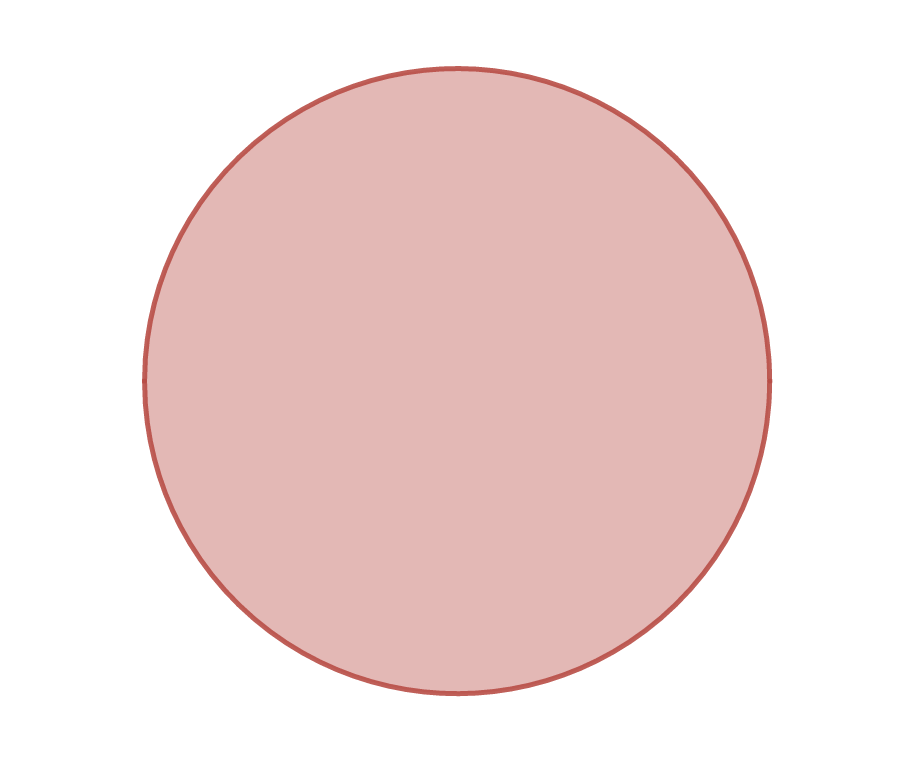
\includegraphics[scale=0.4]{H_0.png}\\
				$H_2$

				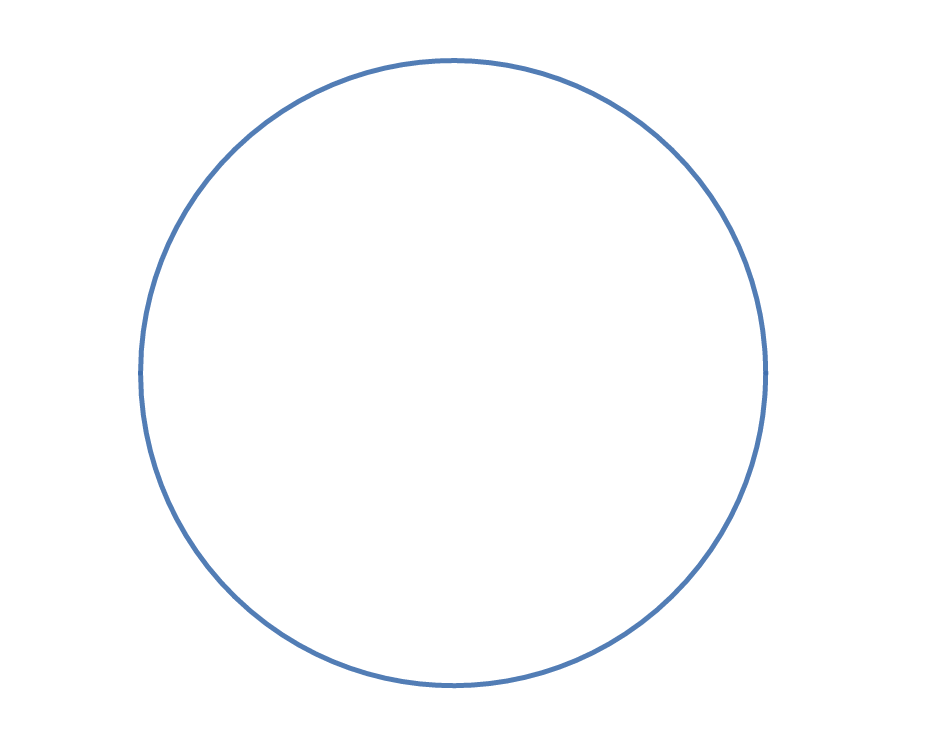
\includegraphics[scale = 0.4]{D_H_0.png}\\
				$\partial_\cA H_2$
		  \end{center}
\end{enumerate}

	As our notation implies, each $n-$handle corresponds to the 2-manifold we attach depending on our Morse index. We can consider each case and give some intuition. Let $f:M\rightarrow \bR$ be a Morse function defined on a closed surface $M$. Suppose $p$ is a critical point of $f$. 
	\begin{enumerate}[(a)]
		\item If the Morse index of $p$ is 0 \\
		Then, we know from the Morse lemma that there is some local coordinate system around $p$ where $f = x^2 + y^2 +f(p)$. We can just set $f(p)=0$, and then in this local coordinate system, $M_{p-\varepsilon} \cong \emptyset$ for all $\varepsilon > 0$, that is, the sublevel set of $M$ at $p$ according to this local coordinate system is the empty set. As we go through our critical point, we see that $M_{p+\varepsilon} \cong H_0$ since the surface defined by $f=x^2+y^2, f\in[0,\varepsilon]$ is diffeomorphic to a 2-disk, our 0-handle. Notice that to this point, we could have actually replaced 0-handle with any $n-$handle and the analysis would technically be correct, but this is where the attachment boundary comes in. We know that the attatchment boundary of $H_0$ is the empty set, exactly what the sublevel of $M$ at $p-\varepsilon$ is, meaning we can ``attach'' a 0-handle. This will make more sense when we have a non-trivial attachment boundary. In conclusion, when we go through a critical point with Morse index equals to 0, we add a 2-disk to our sublevel set, making sure not to attach to anything existing. 
		\item If the Morse index of $p$ is 1\\
		In this case, the Morse lemma tells us we have the form $f = x^2 - y^2$. The graph of this function looks like a saddle, so when we consider the ``restricted'' sublevel set $f \in [-\varepsilon, 0]$, we notice that under this domain, $f$ is diffeomorphic to two disjoint 2-disks. As we pass the critical point, we see that $f \in [0,\varepsilon]$ is differomorphic to just a singular 2-disk, so we know that as we pass the critical point, we need to somehow combine the two disjoint components into a single component. Well, to do so, we can break up the perimeter of our disjoint 2-disks into some $n>2$ arcs and take one arc from each disk to be our lower attachment boundary. Then, we can attach our 1-handle by identifying its attachment boundary to the two arcs. In doing so, we notice that we end up with a ``dumbell'' shape which is indeed diffeomorphic (strictly speaking it is only homeomorphic, but we can apply a smoothing procedure to the attachment to upgrade this to diffeomorphism) to a single 2-disk. 
		\item If the Morse index of $p$ is 2\\
		This case is similar to our first case. The Morse lemma tells us we have the form $f = -x^2-y^2$, an upsidedown paraboloid. Well, any sublevel set below the critical point is diffeomorphic to an annulus, and as we go across the critical point, we once again get a 2-disk. This fits perfectly with how we defined our 2-handle, as we can attach our attachment boundary directly to the inner circumference of the annulus in order to fill out the disk. By this reasoning, we know that we can only attach a 2-handle when our sublevel set has a (disconnected) component of the boundary diffeomorphic to the 1-sphere. 
	\end{enumerate}

	The intuitive way to think about handle attachment is that attaching a 0-handle is just adding a disjoint disk to our surface, attaching a 1-handle is just connecting two locally disconnected components, and attaching a 2-handle is filling a hole to close a component of our manifold. 

	In order to make all the analysis above concrete, we can consider a very simple example, the torus. We will do this more qualitiatively without worrying too much about the exact coordinate charts in order to focus more on handle decomposition. To start, we will take our Morse function to be the the height function of a ``vertical torus'' (as in how a donut would roll). One can easily verify that this is indeed a Morse function, and it has a total of four critical points. Starting at the bottom, we have a critical point with index 0, so handle decomposition tells us to start with a singular 2-disk. Next, we have a critical point of index 1. We might think this is an error since we dont have two connected components in our 2-disk, but this is okay since we only need the components to be \textbf{locally} disconnected. To get these components, we can think of turning our 2-disk into a bowl then just considering two antipodal arcs. Locally, these are disconnected, so we can attach our 1-handle along these arcs. At this point, we have something that is diffeomorphic to a cylinder. Our next critical point also has index 1. This time, our boundary actually has two disconnected components, so we can just attach our 1-handle normally. Now, as we expect, we have something which is diffeomorphic to a torus with a 2-disk removed. This hole gets filled in by our final critical point, which has index 2 in order to recover our torus! 

\subsection{Existence of Morse Functions}

	To conclude this section, we will give the theorem which promises the existence of Morse functions on certain manifolds, and give a very rough proof outline. 

	\begin{theorem}
		Let $M$ be a closed $n-$manifold and $f:M\rightarrow \bR$ a smooth function defined on $M$. Then, for all $\varepsilon >0$, there exists a Morse function $h:M\rightarrow \bR$ defined on $M$ such that $h$ is $\varepsilon-C^2$ close to $f$, that is, the zeroth, first, and second derivatives of $f$ and $h$ at any point are within $\varepsilon$ of each other. 
	\end{theorem}

	This theorem promises not only the existence of Morse functions on any closed manifold, but arbitrarily many Morse functions. The idea behind the proof is as follows. 

	We start with the given smooth function $f$ defined on our manifold. If each of $f$'s critical points are already non-degenerate, then it is a Morse function and we are done, so we can assume there is at least one degenerate critical point. Now, we can perturb $f$ slightly in various ways until we remove this degeneracy. The important idea here is that non-dedegenerate critical points stay non-degenerate under small perturbations, but degenerate critical points are ``unstable'', and so may split into multiple critical points or just disappear completely under small perturbations. We can repeat this process until we eventually end up with a function $h$ for which all the critical points are non-degenerate, and by setting conditions on how we perturb our original function, we can make sure $h$ is $\varepsilon-C^2$ close to $f$. 
\section{Application to Euler Characteristic}

In this section, we will show how we can apply Morse theory in order to extract an important topological invariant without knowing anything about how our surface looks like. 
\subsection{Simplicial n-Complexes and Euler Characteristic}
We start with some definitions and theorems. 

\begin{definition}[Simplicial 1,2-Complex]
	A \textbf{simplicial 1-complex} is a topological space consisting of points and line segments, identified by verticies and along edges. 

	A \textbf{simplicial 2-complex} is a topological space consisting of points, line segments, and triangles identified along verticies and edges. 
\end{definition}

\textbf{Examples and Non-examples}
\begin{example}
	The following are all simplicial 2-complexes:
	\begin{enumerate}
		  \item A point
		  \item A line segment between two points
		  \item A triangle consisting of three line segments connecting three points
	\end{enumerate}
\end{example}

\begin{definition}[Euler Characteristic]
	The \textbf{Euler characteristic} $\chi$ of a simplicial 2-complex is given by the formula 
	\begin{center}
		  $\chi = V-E + F$
	\end{center}
	where $V$ is the number of verticies, $E$ is the number of edges, and $F$ the number of triangles (faces). 
	
\end{definition}

We will be using the following two theorems without including proofs.

\begin{theorem}
	If $P_1, P_2$ are homeomorphic simplicial 2-complexes, then $\chi(P_1) = \chi(P_2)$
\end{theorem}

\begin{theorem}
	Every compact n-manifold $M$ is homeomorphic to a simplicial n-complex $P$. We can define $\chi(M) := \chi(P)$. 
\end{theorem}

And one which we will quickly prove. 

\begin{theorem}
	Let $P,Q$ be two disjoint simplicial n-complexes, then we have that 
	\begin{center}
		  $\chi(P\sqcup Q) = \chi(P) + \chi(Q)$. 
	\end{center}
\end{theorem}

\begin{proof}
	Let $(V_1,E_1,F_1) \subset \bN^3$ be the number of verticies, edges, and faces of $P$, $(V_2,E_2,F_2)$ that of $Q$. Then, since $Q \cap P = \emptyset$, we have that the total number of verticies of $Q\sqcup P$ is $V_1+V_2$, and the same goes for $\#$ edges and faces. Thus we get $\chi(P\sqcup Q) = V_1 +V_2 -(E_1+E_2)+F_1+F_2 = V_1-E_1+F_1 + V_2-E_2+F_2 = \chi(P) +\chi(Q)$. 
\end{proof}

\subsection{Euler Characteristic from Morse Theory}


\noindent
In the context of Morse theory on surfaces, we can look for simplicial 2-complexes homeomorphic to 0,1,2-handles and their ``attachment boundaries'' in order to extract information about their Euler characteristics. 

\begin{enumerate}
      \item \textbf{0-Handle}\\
            The 0-handle is homeomorphic to a (filled) triangle, so $\chi(H_0) = 3 - 3 + 1 = 1$. Similarly, $\chi(\partial_\cA H_0) = 0-0+0 = 0$. 
			\begin{center}
				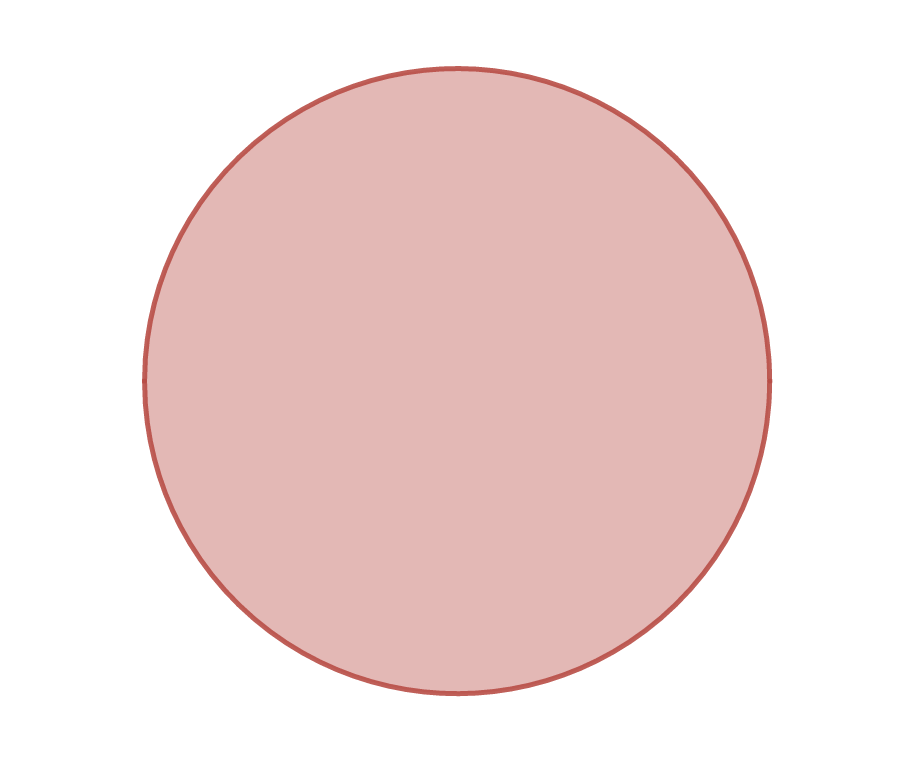
\includegraphics[scale=0.4]{H_0.png} 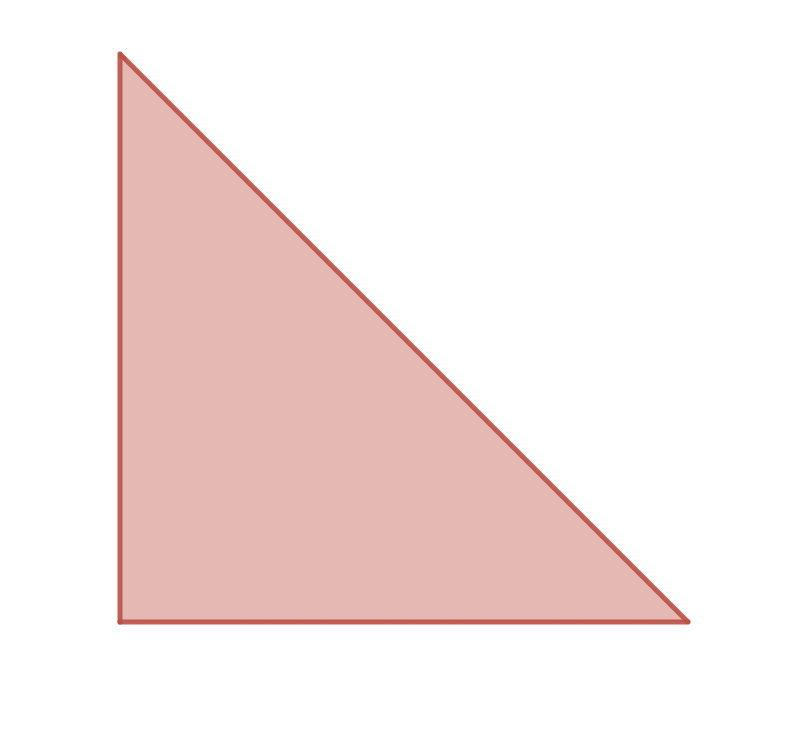
\includegraphics[scale=0.4]{triangle.png} \\
				$H_0 \cong D^2 \cong $ Triangle
				
		  \end{center}
      \item \textbf{1-Handle}\\
            A 1-handle is also homeomorphic to the 2-disk, but another way to determine its Euler characteristic is by considering it as two (congruent, equilateral) triangles with one coincident edge. This gives $\chi(H_1) = 4 - 5+ 2 = 1$. The attachment boundary $\partial H_1$ is just given by two disjoint sets of two verticies and one edge connecting them, giving us $\chi(\partial_\cA H_1) = 4 - 2 + 0 = 2$. 
            \begin{center}
                  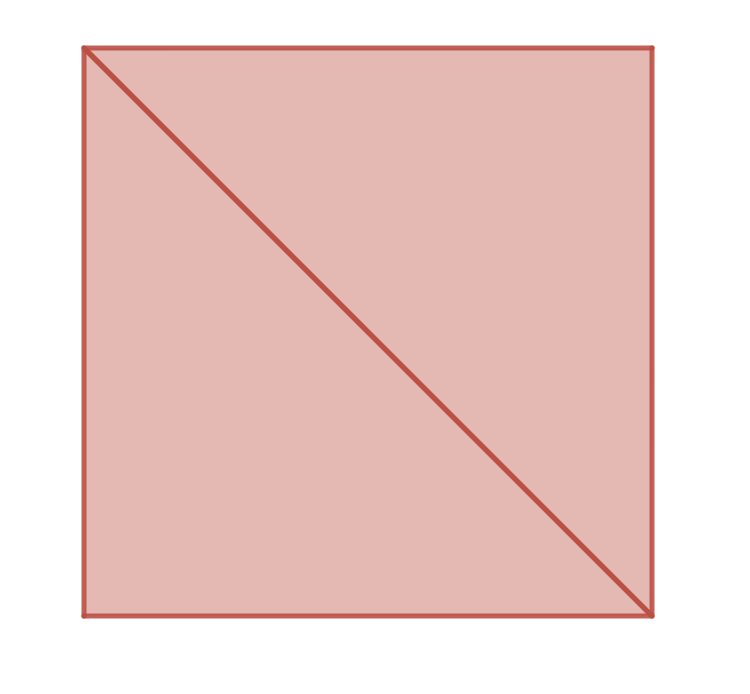
\includegraphics[scale=0.5]{square.png} \\
                  $H_1 \cong D^1\times D^1$

                  
\includegraphics[scale = 0.5]{D_H_1.png}\\
                  $\partial_\cA H_1 \cong D^1 \sqcup D^1$
            \end{center}
      \item \textbf{2-Handle}\\
            A 2-handle $H_2$ is homeomorphic to the 2-disk, so $\chi(H_0) = 3 - 3 + 1 = 1$. Similarly, $S^1$ is homeomorphic to three verticies connected by 3 edges, ie. the perimeter of a triangle, so $\chi(\partial_\cA H_0) = 3-3+0 = 0$. 
            \begin{center}
                  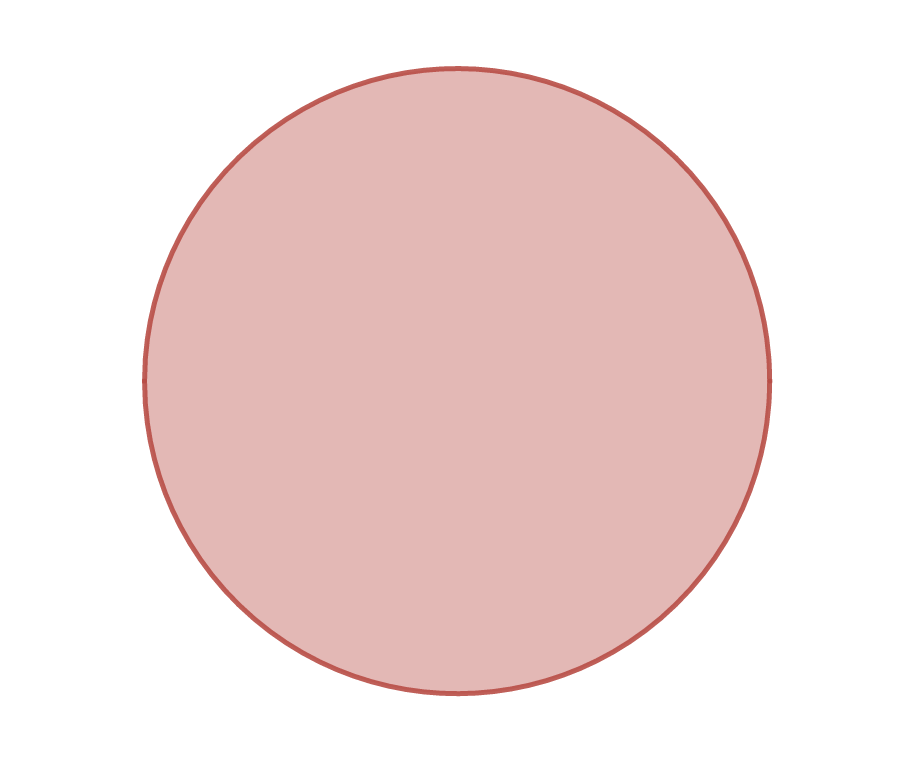
\includegraphics[scale=0.4]{H_0.png} 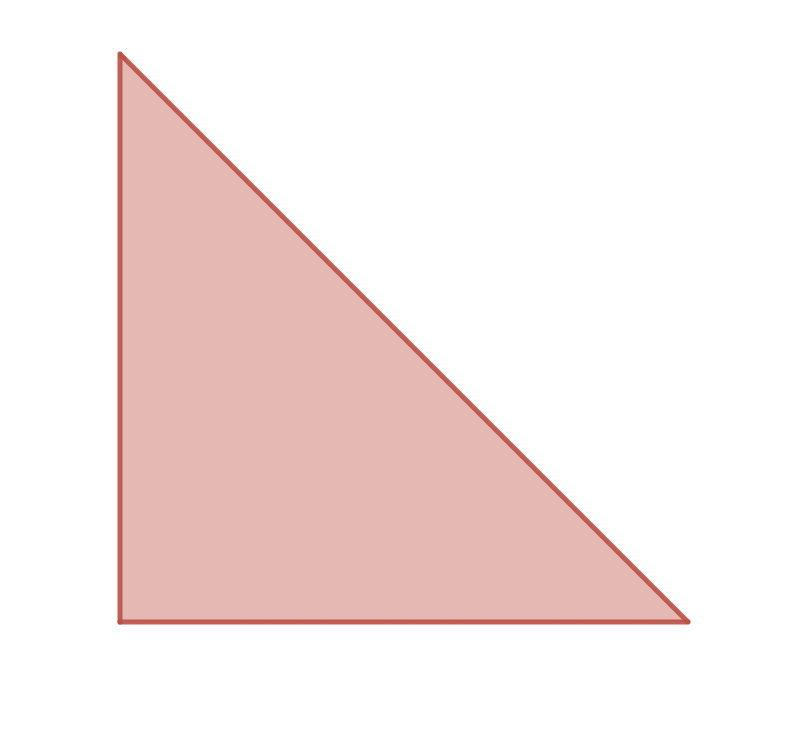
\includegraphics[scale=0.4]{triangle.png} \\
                  $H_2 \cong D^2 \cong $ Triangle

                  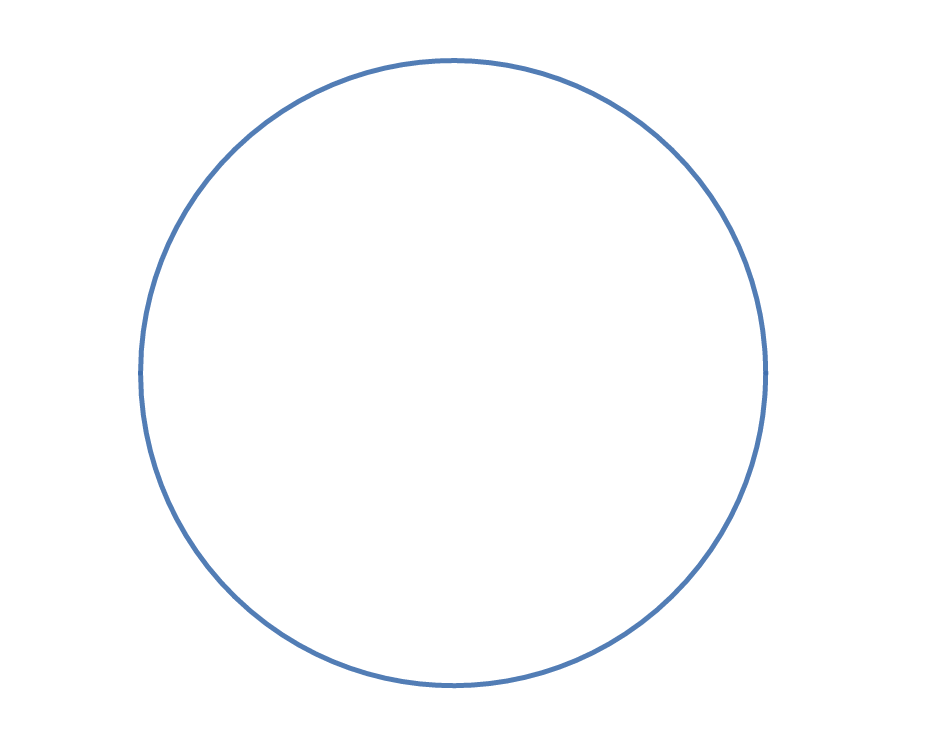
\includegraphics[scale = 0.4]{D_H_0.png}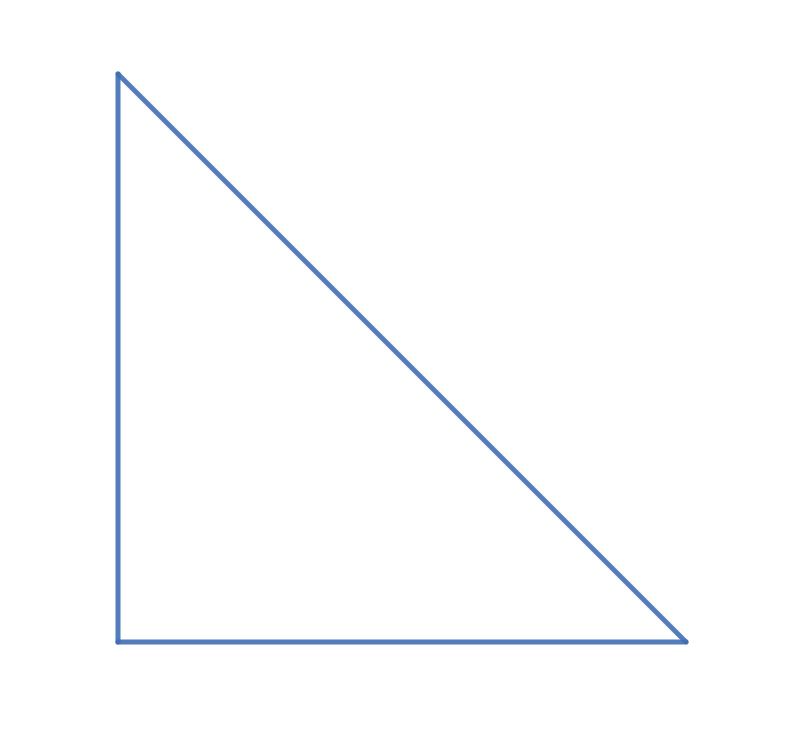
\includegraphics[scale=0.4]{perimeter.png}\\
                  $\partial_\cA H_2 \cong S^1 \cong$ Perimeter of a Triangle
            
            \end{center}
\end{enumerate}

Now we can give the proof of the main result:
\begin{proof}
      Let $M \subset \bR^3$ be a compact manifold which exhibits a Morse function $f:M \rightarrow \bR$. Let $(i_1,i_2,...,i_n)\in \{0,1,2\}^n$ denote the Morse indicies of the $n$ (non-degenerate) critical points $\{p_1,p_2,...,p_n\}$ of $f$. By the handle decomposition theorem, we know that $M$ is homeomorphic to the union of $A$ 0-handles, $B$ 1-handles, and $C$ 2-handles, where $A = \# \{i_j : i_j = 0\}, B = \# \{i_j : i_j = 1\}, C= \# \{i_j: i_j = 2\}$. To prove our desired result, we will split into cases of observing what happens to the Euler characteristic upon attaching a 0,1, or 2-handle. In each of the following cases, we will let $M_{p} = \{x \in M: f(x)\leq f(p)\}$, i.e. the sublevel set of $M$ at $p$. Note that the boundary $\partial M_{p} = \{x \in M : f(x) = f(p)\}$. 
      
      \begin{enumerate}
            \item $i_j = 0$\\
            In the case that our morse index is 0, we are simply taking the disjoint union $M_{p_{i_j}} \sqcup H_0$, so we can use our additivity property to get that $\chi(M \sqcup H_0) = \chi(M) + \chi(H_0) = \chi(M) + 1$. 

            \item $i_j = 1$\\
            Attaching a 1 handle is slightly more complicated. First, $M_{p_{i_j}}$ is homeomorphic to some simplicial 2-complex $\cS_M$ with $V_M$ verticies, $E_M$ edges, and $F_M$ faces. Furthermore $\partial M_{p_{i_j}}$ is homeomorphic to some simplicial 1-complex $\cS_j$ with $V_j$ verticies and $E_j$ edges, where $\cS_j \subseteq \cS_M$. We claim that we can assume that there are two distinct edges $E_1, E_2$ such that their endpoints (verticies called, say $V_1, V_1'$ and $V_2,V_2'$) are also distinct. We are free to assume this since the simplicial complex $\cS_j'$ created by adding verticies at the midpoints of each edge and ``splitting'' the original edge into two edges is homeomorphic $\cS_j$. In practice, this data will be guaranteed by the fact that our Morse function behaves as it does. 
            \begin{center}
                  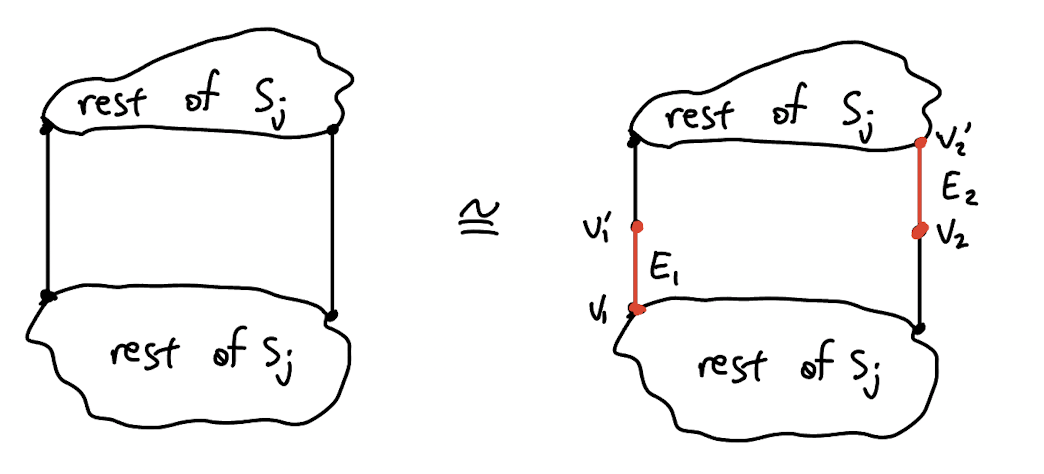
\includegraphics[scale = 0.4]{sim.png}
            \end{center}
            Now that we have a subset of $\cS_j$ which is homeomorphic to the attachment boundary $\partial_\cA H_1$, we can attach the handle to the boundary by identifying the respective edges and verticies. Concretely, our 1-handle $H_1$ is homeomorphic to a simplicial 2-complex with $V_H = 4, E_H = 5, F_H = 2$ with attachment boundary $\partial_\cA H_1$ homeomorphic to a simplicial 1-complex with $V_\partial = 4, E_\partial = 2$. We can identify these homeomorphic parts of the ``upper and lower'' attachment boundaries and we can recount the total number of verticies, edges, and faces to get the resulting Euler characteristic. Clearly, the number of faces is just the sum of the two parts, since we don't identify any faces, i.e. $F_{M\cup H_1} = F_M + F_H = F_M + 2$. Next, since we are now identifying 4 verticies of $H_1$ with those on $S_j$, we get that $V_{M\cup H_1} = V_M + V_H - 4 = V_M + 4 - 4 = V_M$ to account for double counting. Finally, we get something similar for the number of edges, namely $E_{M\cup H_1} = E_M + E_H - 2 = E_M + 5 - 2 = E_M + 3$. To get the Euler characteristic, we apply our formula to get $\chi(M \cup H_1) = V_M - E_M - 3 + F_M + 2 = V_M - E_M+ F_M -1 = \chi(M)-1$
            

            \item $i_j = 2$\\
            In order to even attach a 2-handle to $M_{p_{i_j}}$, we necessarily require that there be a connected component of $\partial M_{p_{i_j}}$ which is homeomorphic to $S^1$. Because the attachment boundary of $H_2$ is also exactly $S^1$ (which is homeomorphic to a triangle), we can identify the two circle coincidently as simplicial 1-complexes. This gives us that $V_{M\cup H_2} = V_M + V_H - V_H = V_M$, since all verticies of $H_2$ are on its boundary. A similar statement holds for the edges of $H_2$, so we get $E_{M\cup H_2} = E_M + E_H - E_H = E_M$. As for faces, since we are only identifying the edges and verticies as subsets of the simplicial 2-complexes, the resulting number of faces is just the sum of the two parts, $F_{M\cup H_2} = F_M + F_H = F_M + 1$. Counting, we get $\chi(M\cup H_2) = V_M -E_M + F_M +1 = \chi(M) + 1$. 
      \end{enumerate}

      From the above results, we see that we add 1 to our Euler characteristic everytime we attach a 0 or 2-handle, and subtract 1 everytime we attach a 1-handle, so 
      \begin{center}
            $\chi(M) = A-B+C$. 
      \end{center}
\end{proof}

\section{Acknowledgements}

Professor McFeely Jackson Goodman was the advisor for this project and gave great guidance and intuition for this independent study. 

\end{document}